\appendix

\chapter{Numerical Results}
\thispagestyle{myheadings}

All of the figures are from the code written as a companion to this thesis (see \cite{code}).
The details needed to reproduce the program and the results are given in the repository.
Essentially it consists of a FreeFem++ program (see \cite{freefem}) which handles the MFS and gradient descent, a program that visualizes the mesh, and a program that connects them.
The controller program also has the ability to run multiple processes of the main program in parallel, and saves the outputs.
We highly recommend creating a Docker image in order to reproduce the results rather than creating a similar environment, as FreeFem++ can run on any popular Operating System while the visualization software and the parallel package are both only available on Linux systems.

The polygons in Figures A.1-3 are the domains obtained by the program alongside the information in the table, where the coloring is the (normalized) eigenfunction.
It is notable how quickly the polygons start to look like circles, and with the trend seen in the first eigenvalues the Pólya-Szegő conjecture seems extremely intuitive.
In Table A.1, we list the three different minimization values considered previously, the standard deviation and max difference of both the side lengths and the internal angles, as well as the first eigenvalue and the area of the polygon which minimizes $\left\{ |\Omega| \lambda_{1}(\Omega) \right\} $.
We have also included the corresponding eigenvalue for the minimization problem with area constraint, namely, when $| \Omega | = \pi$.
There are papers which give numerical estimations for the eigenvalues when $N \leq 15$ (see \cite{freitas},\cite{oudet}).
We will give results for polygons with $N \leq 23$, which is a new upper bound for numerical approximations.

\newgeometry{paper=a4paper, left=1.5in,right=1in,top=1in,bottom=1in, footskip=0.25in}

\begin{figure}[hbt!]
    \centering
    \subfloat[N = 3]{
        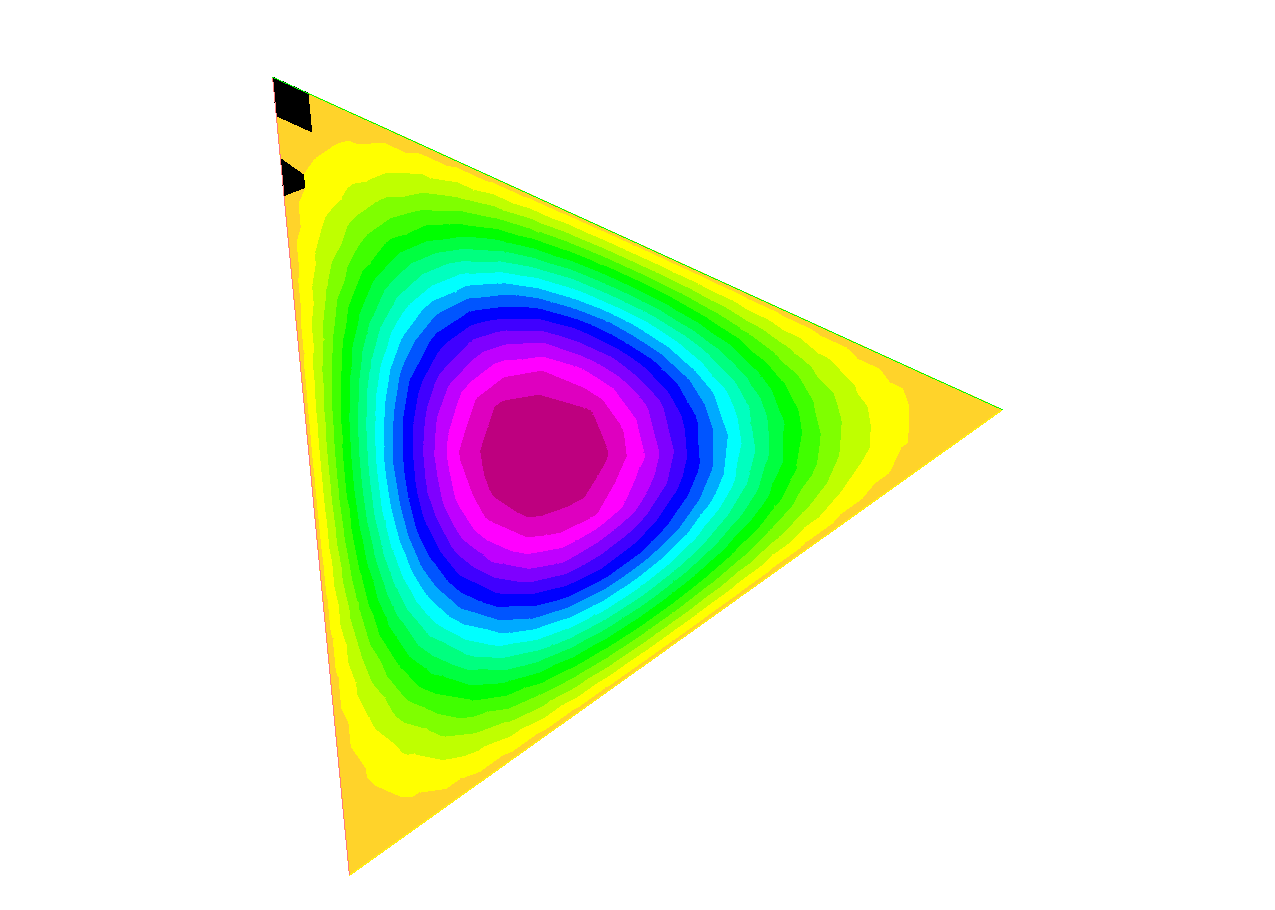
\includegraphics[width=0.5\textwidth]{3sides}
    }
    \subfloat[N = 4]{
        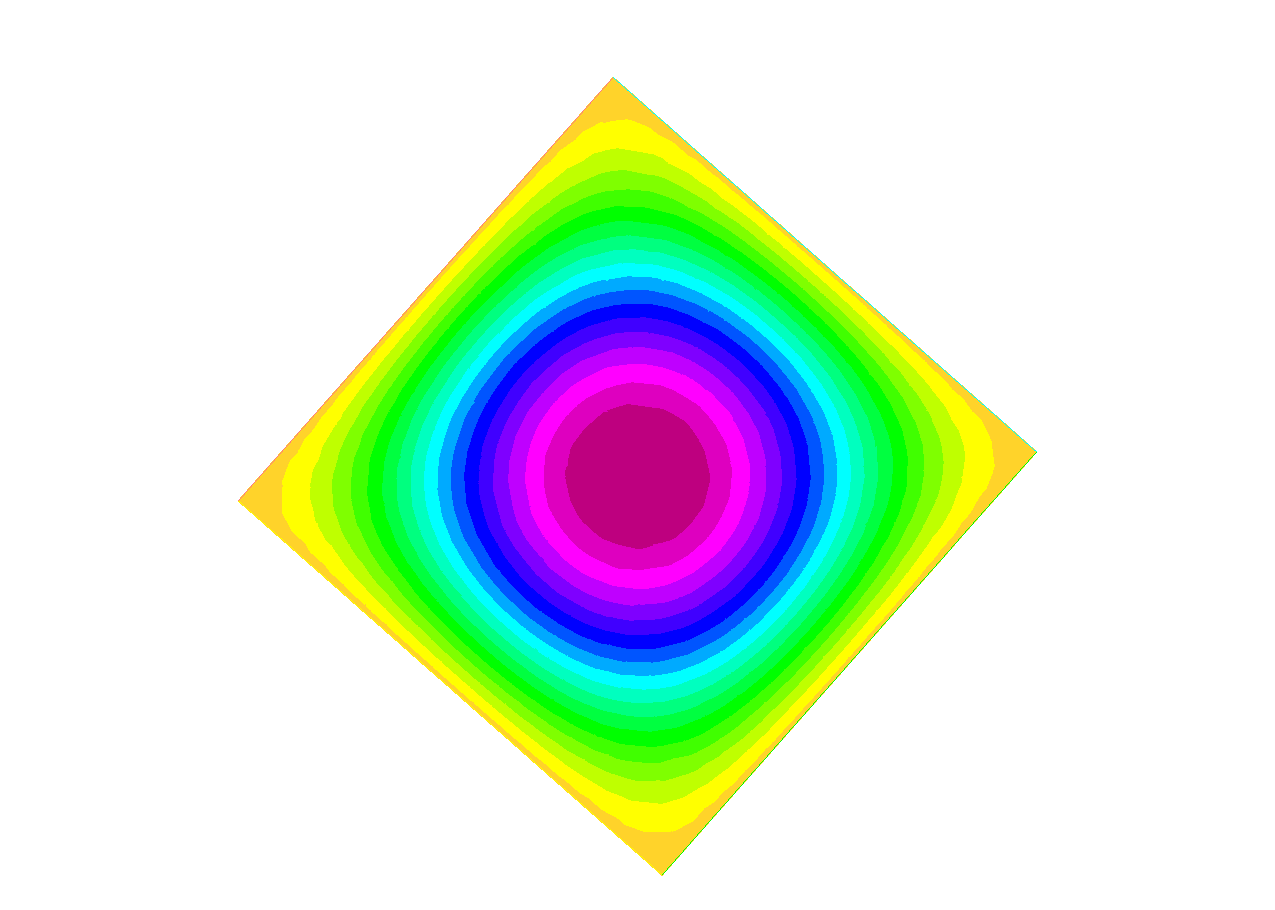
\includegraphics[width=0.5\textwidth]{4sides}
    }

    \subfloat[N = 5]{
        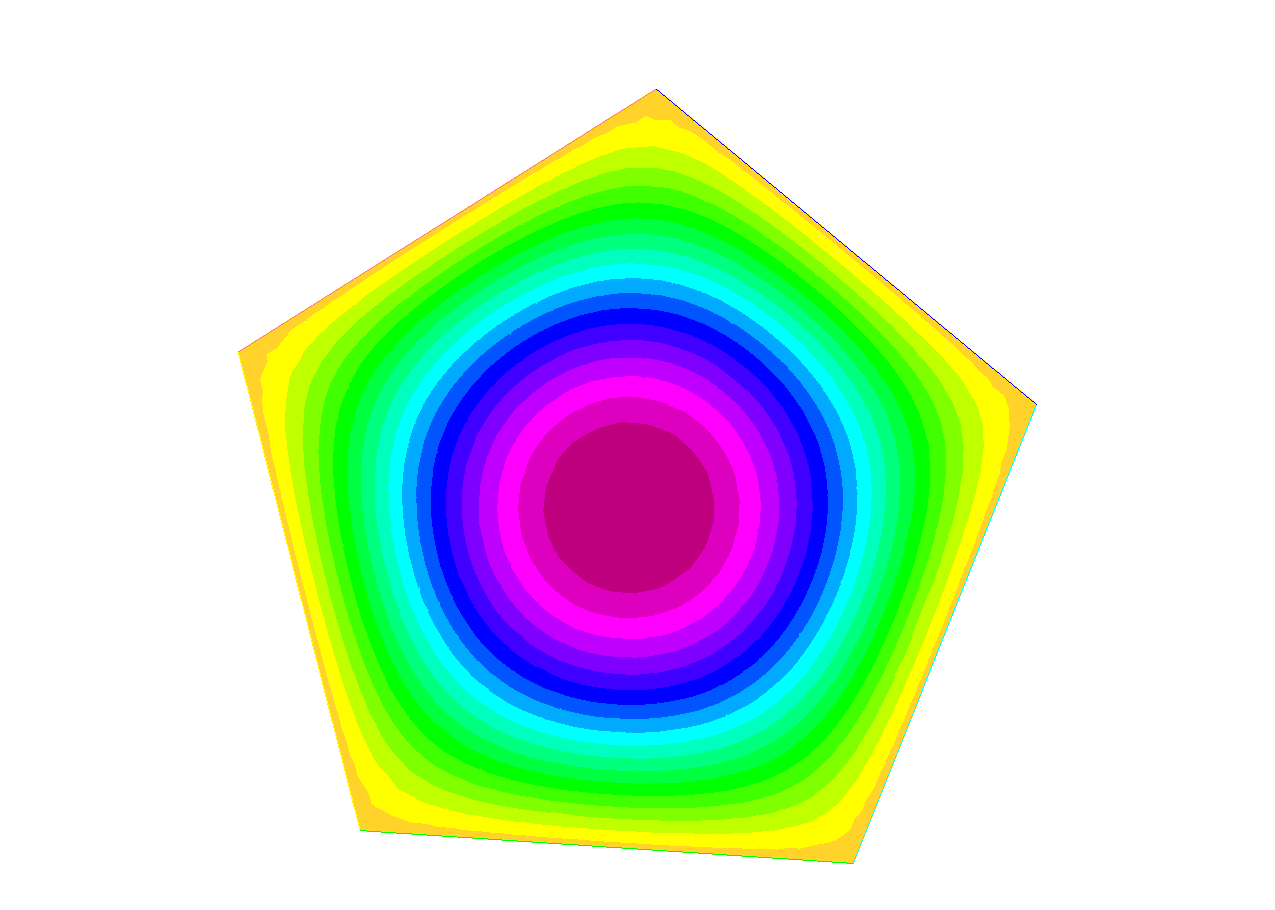
\includegraphics[width=0.5\textwidth]{5sides}
    }
    \subfloat[N = 6]{
        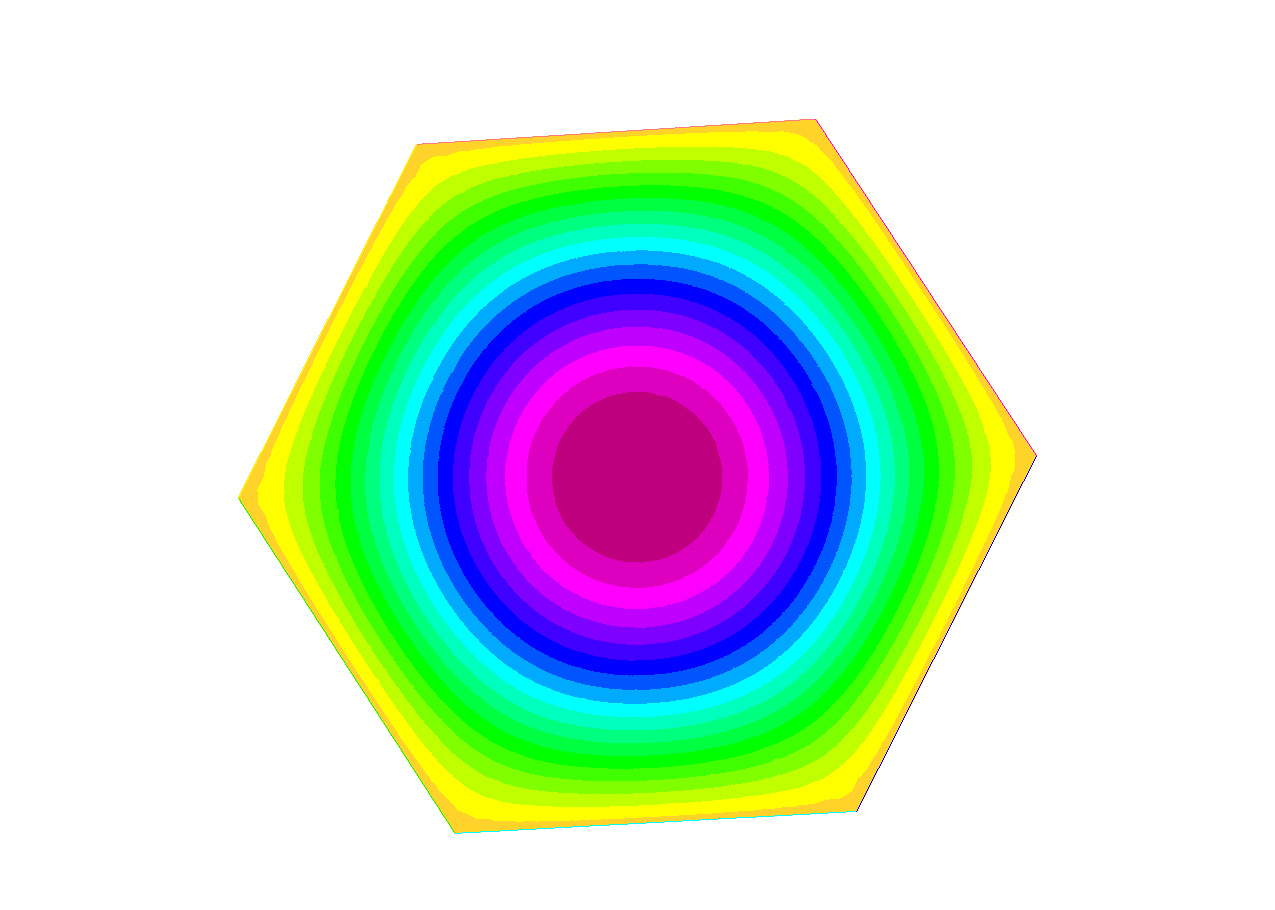
\includegraphics[width=0.5\textwidth]{6sides}
    }

    \subfloat[N = 7]{
        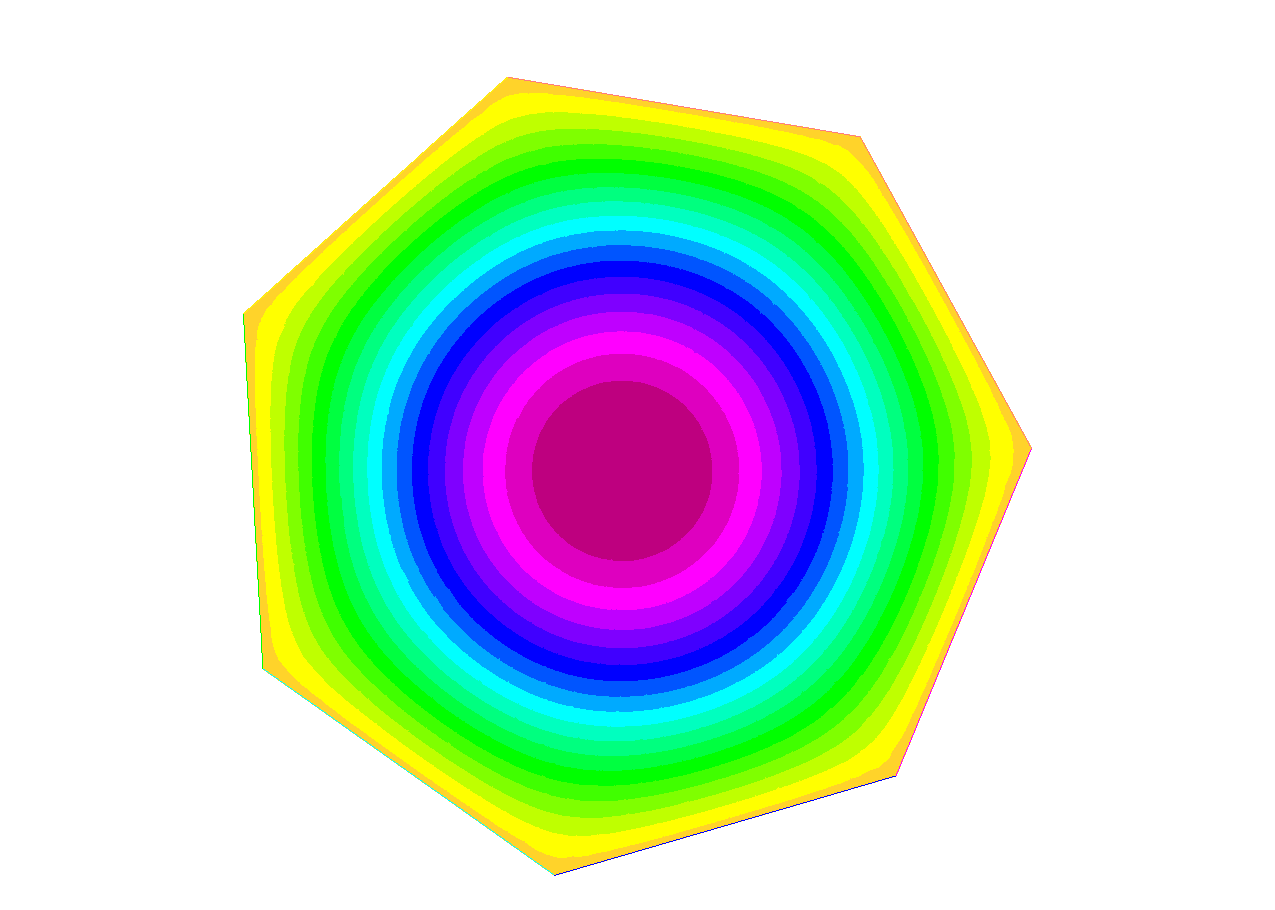
\includegraphics[width=0.5\textwidth]{7sides}
    }
    \subfloat[N = 8]{
        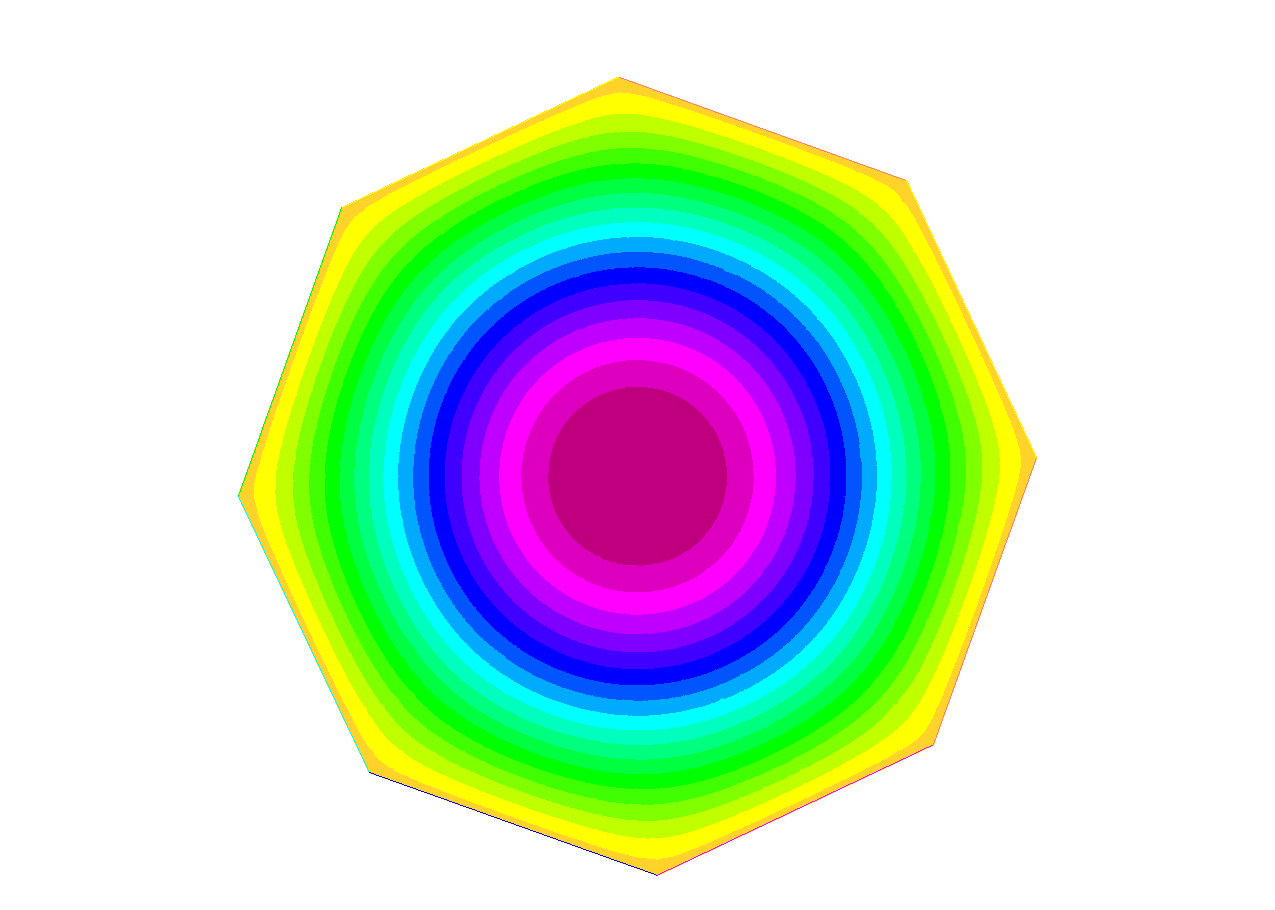
\includegraphics[width=0.5\textwidth]{8sides}
    }

    \subfloat[N = 9]{
        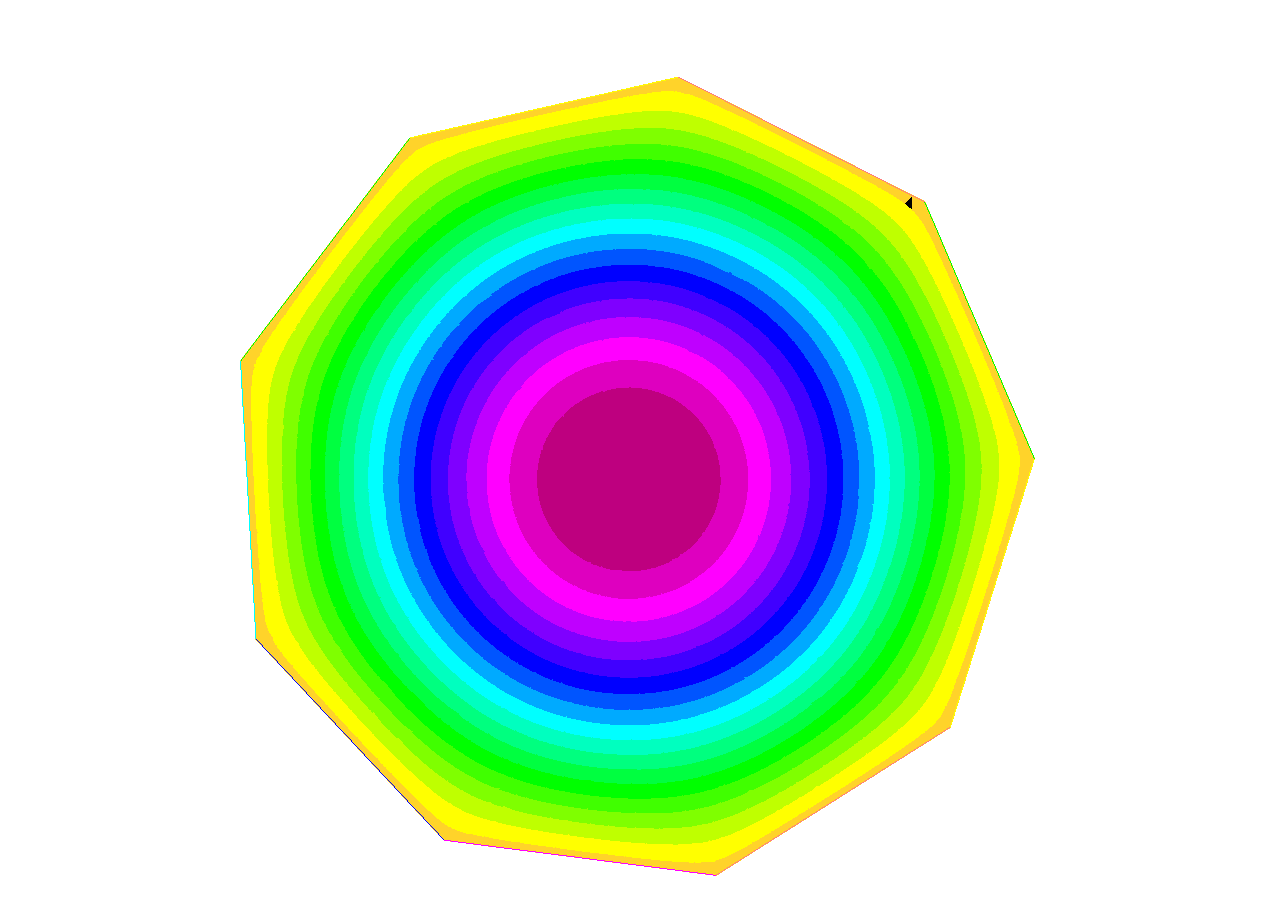
\includegraphics[width=0.5\textwidth]{9sides}
    }
    \subfloat[N = 10]{
        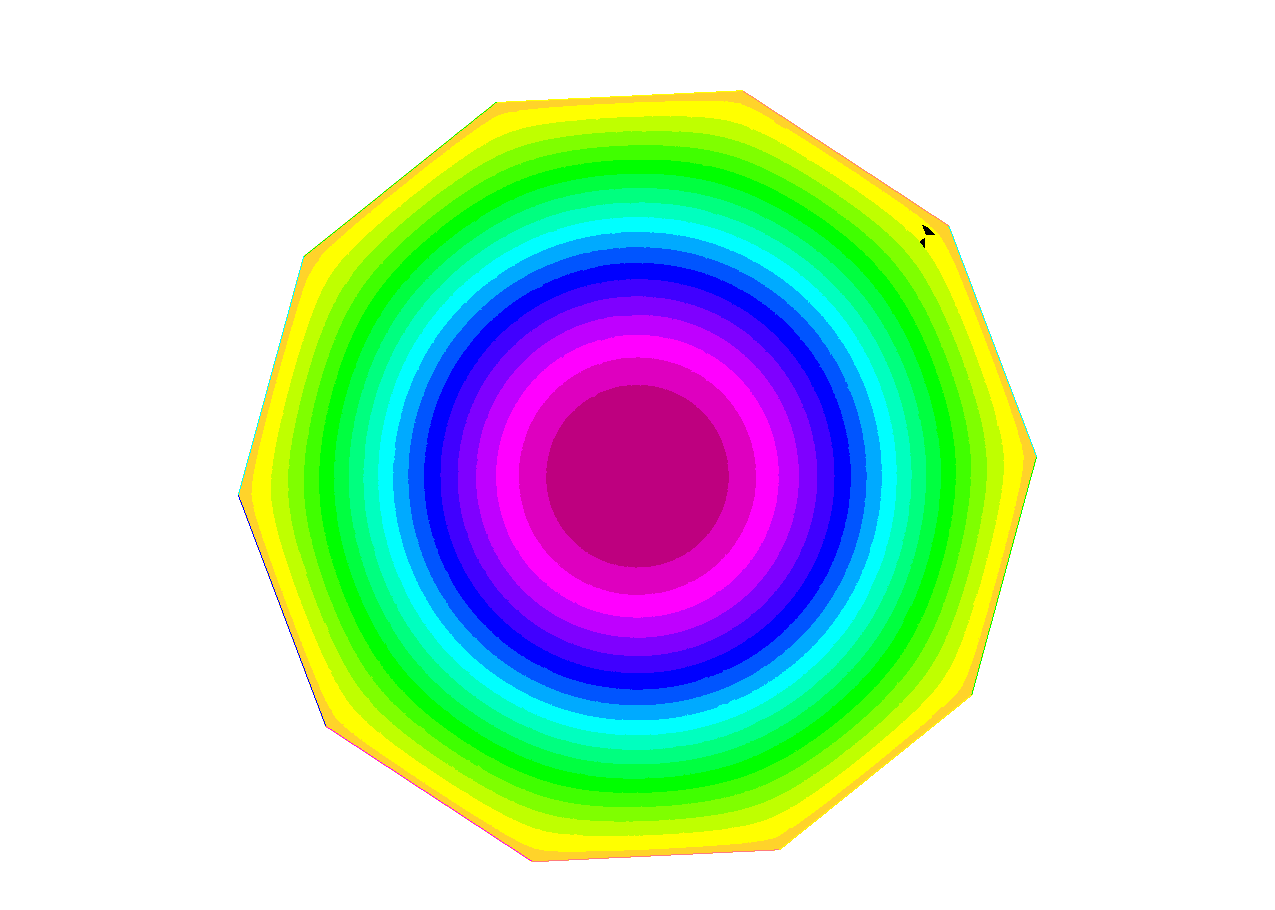
\includegraphics[width=0.5\textwidth]{10sides}
    }
    \caption{Domains and Eigenfunctions Obtained after $1000$ Iterations}
\end{figure}




\begin{figure}[hbt!]
    \centering
    \subfloat[N = 11]{
        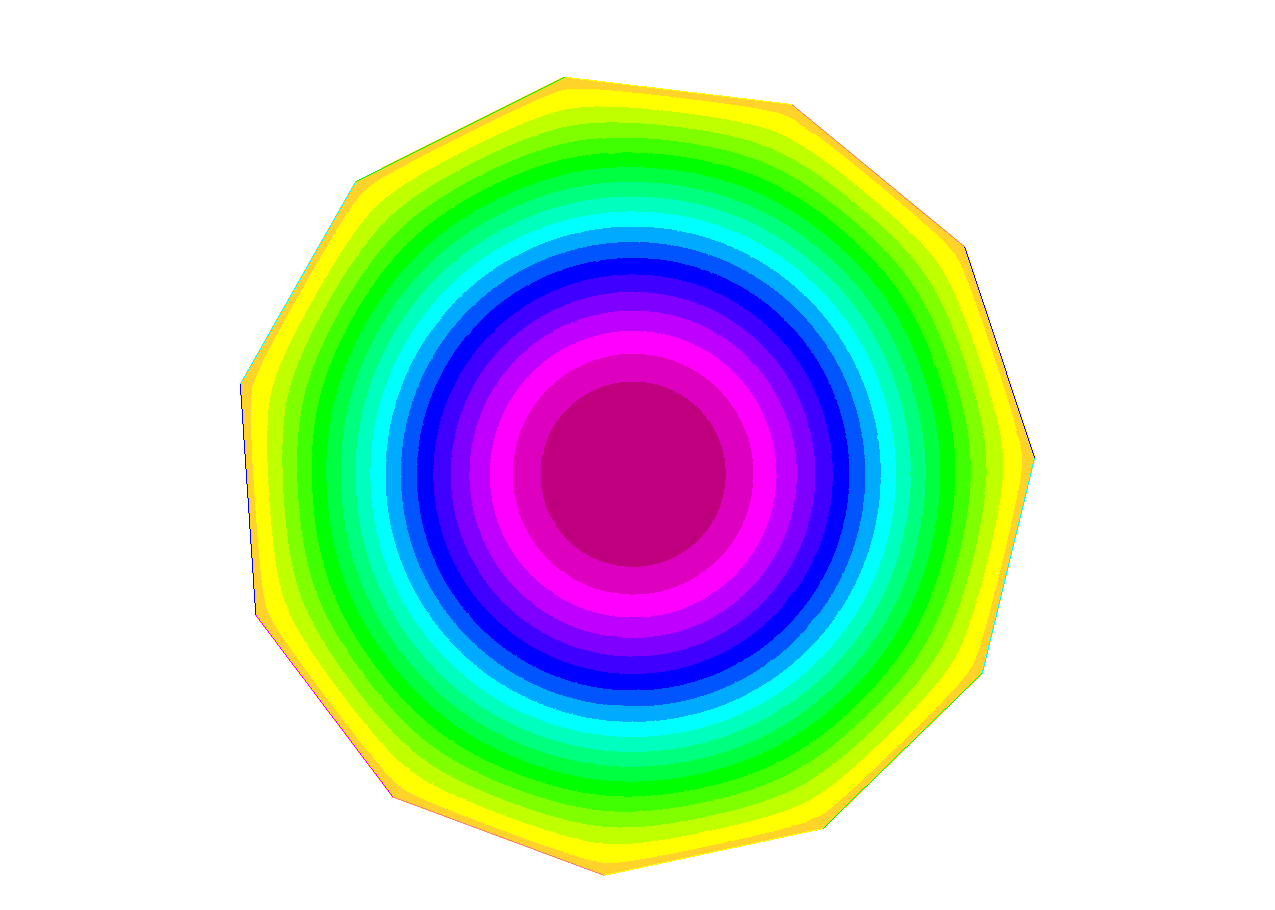
\includegraphics[width=0.5\textwidth]{11sides}
    }
    \subfloat[N = 12]{
        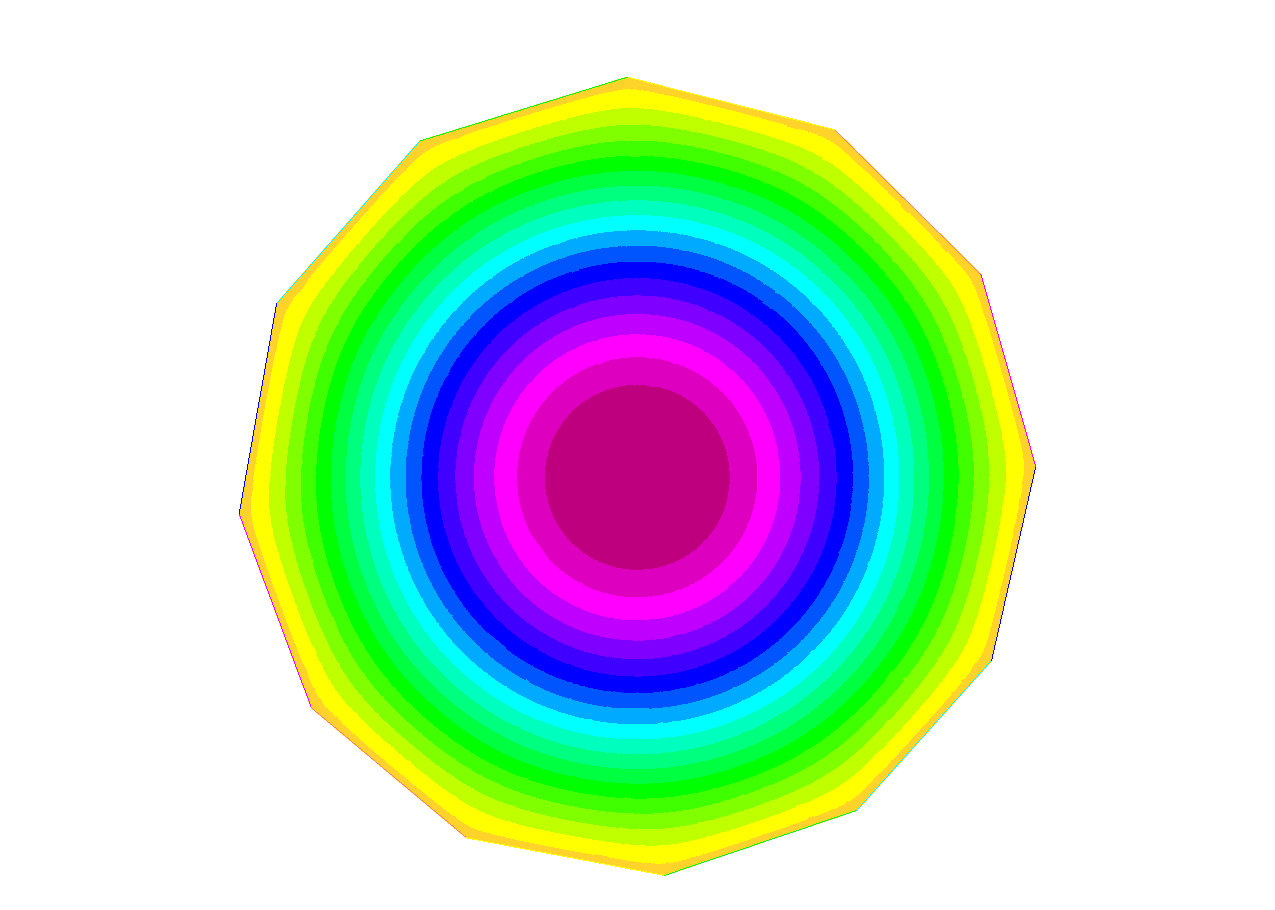
\includegraphics[width=0.5\textwidth]{12sides}
    }

    \subfloat[N = 13]{
        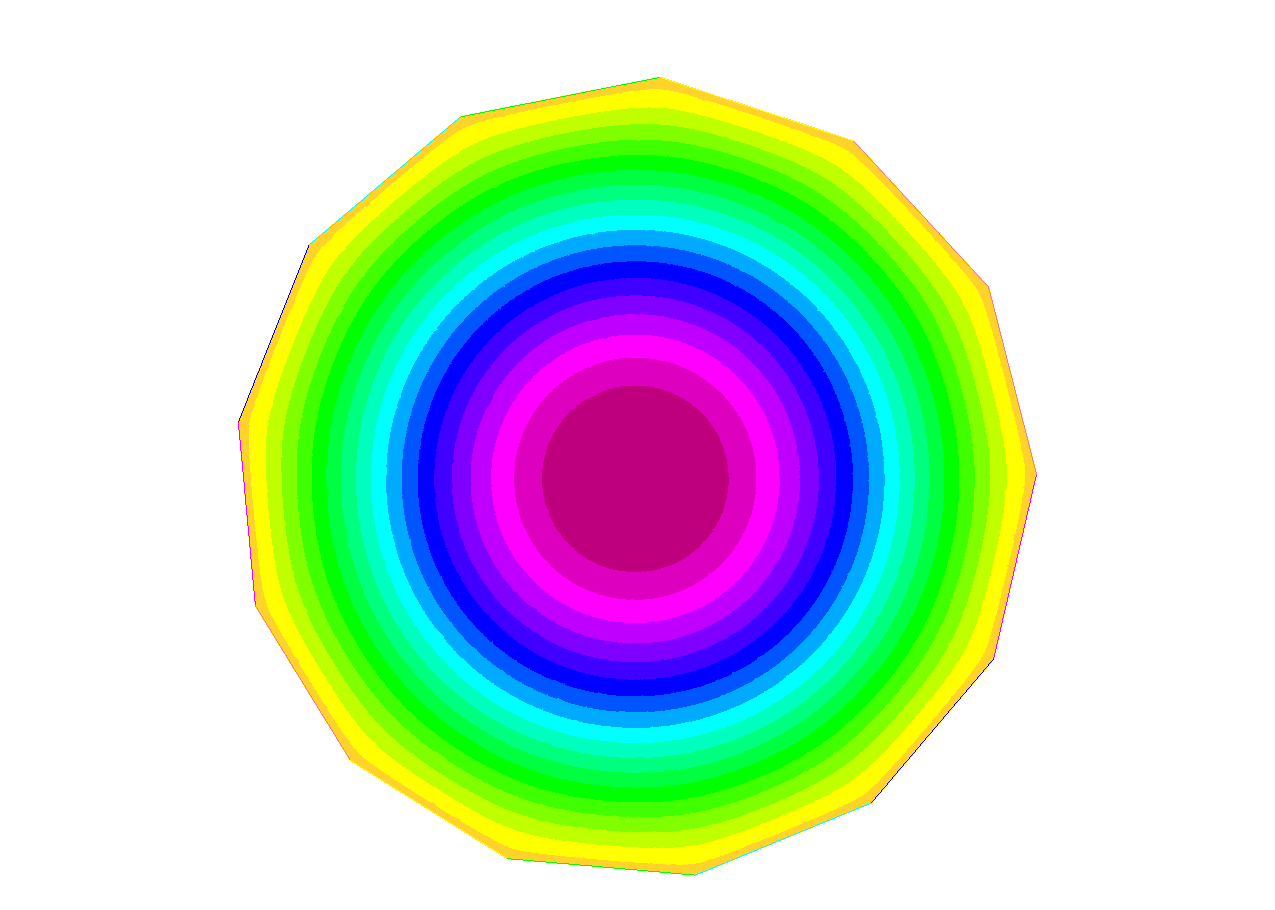
\includegraphics[width=0.5\textwidth]{13sides}
    }
    \subfloat[N = 14]{
        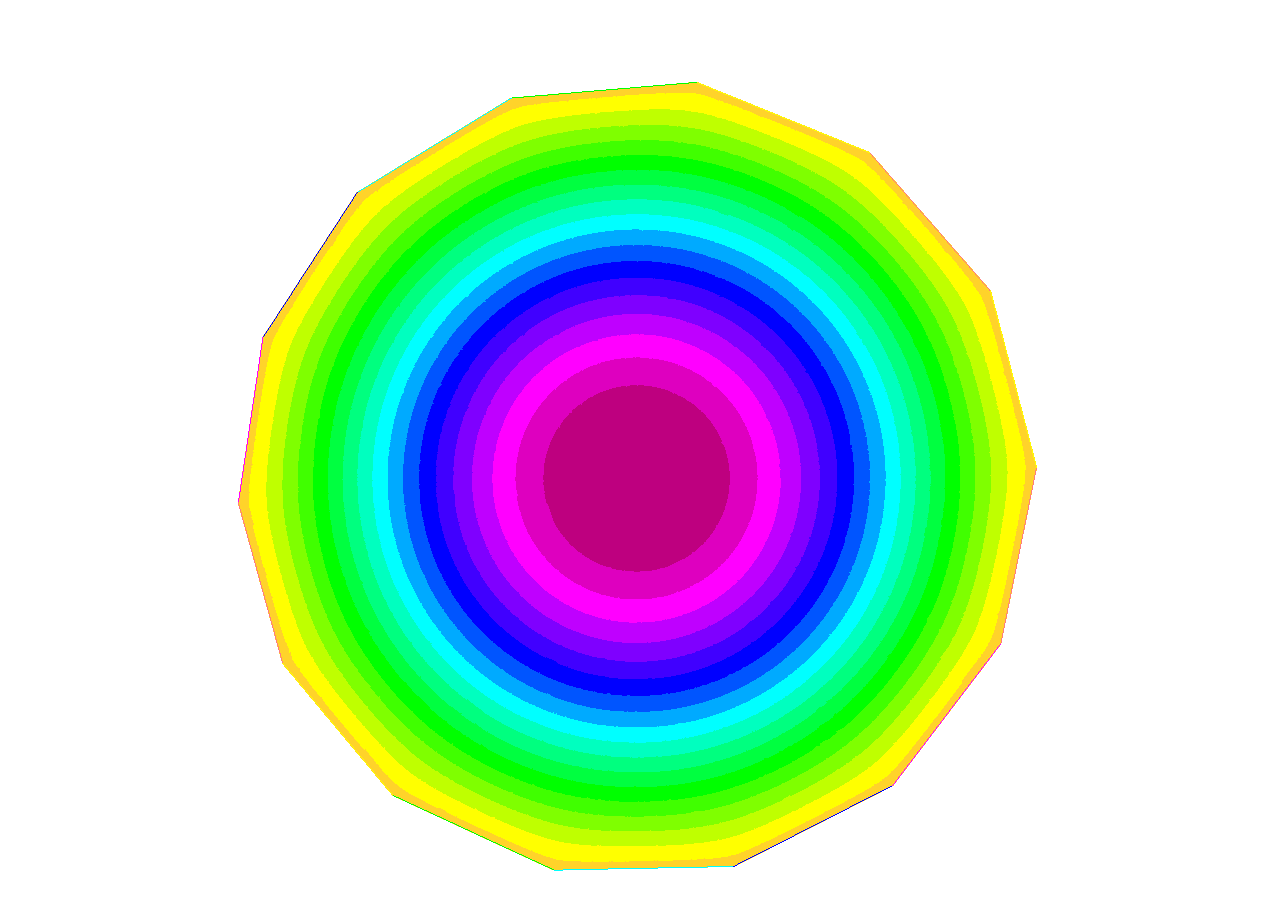
\includegraphics[width=0.5\textwidth]{14sides}
    }

    \subfloat[N = 15]{
        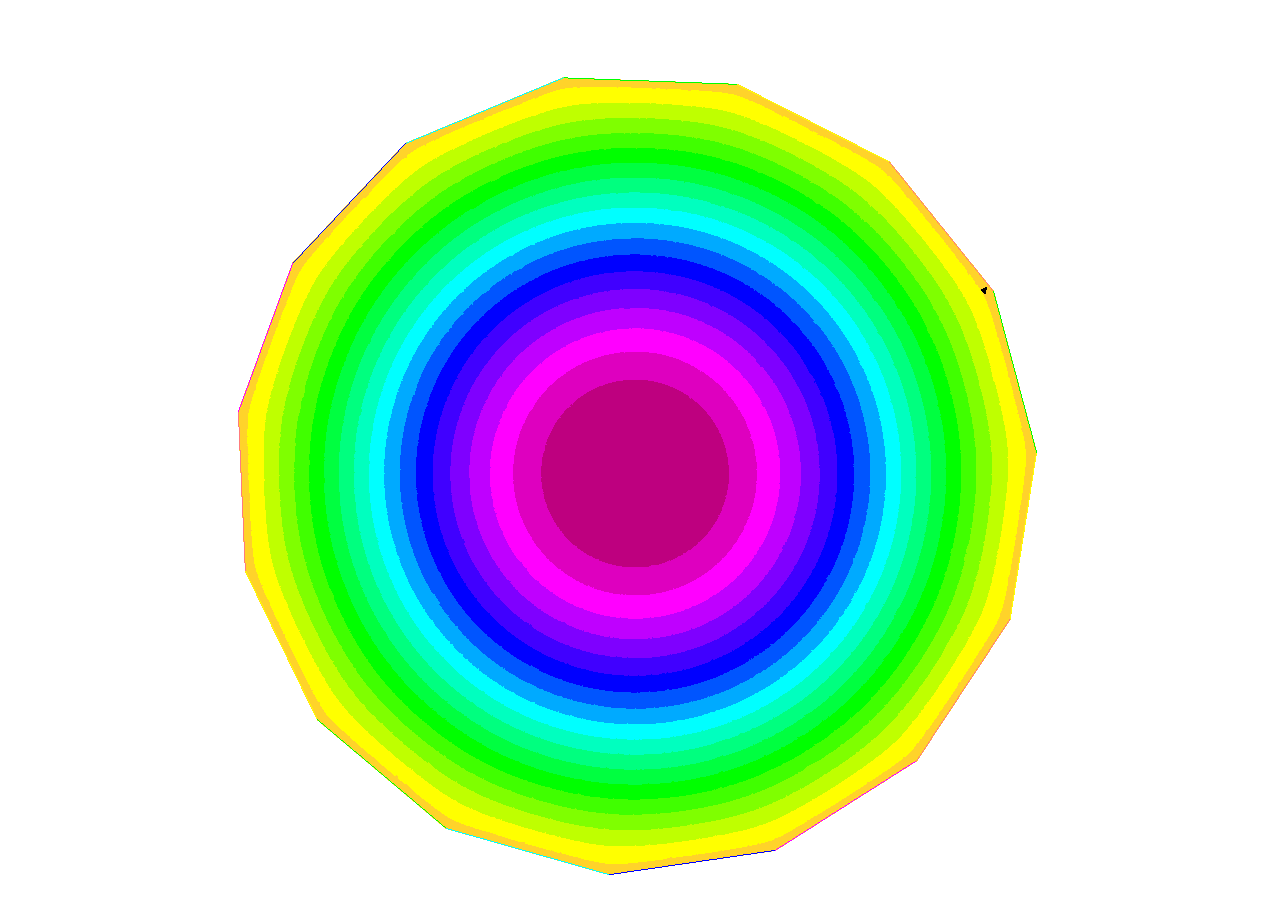
\includegraphics[width=0.5\textwidth]{15sides}
    }
    \subfloat[N = 16]{
        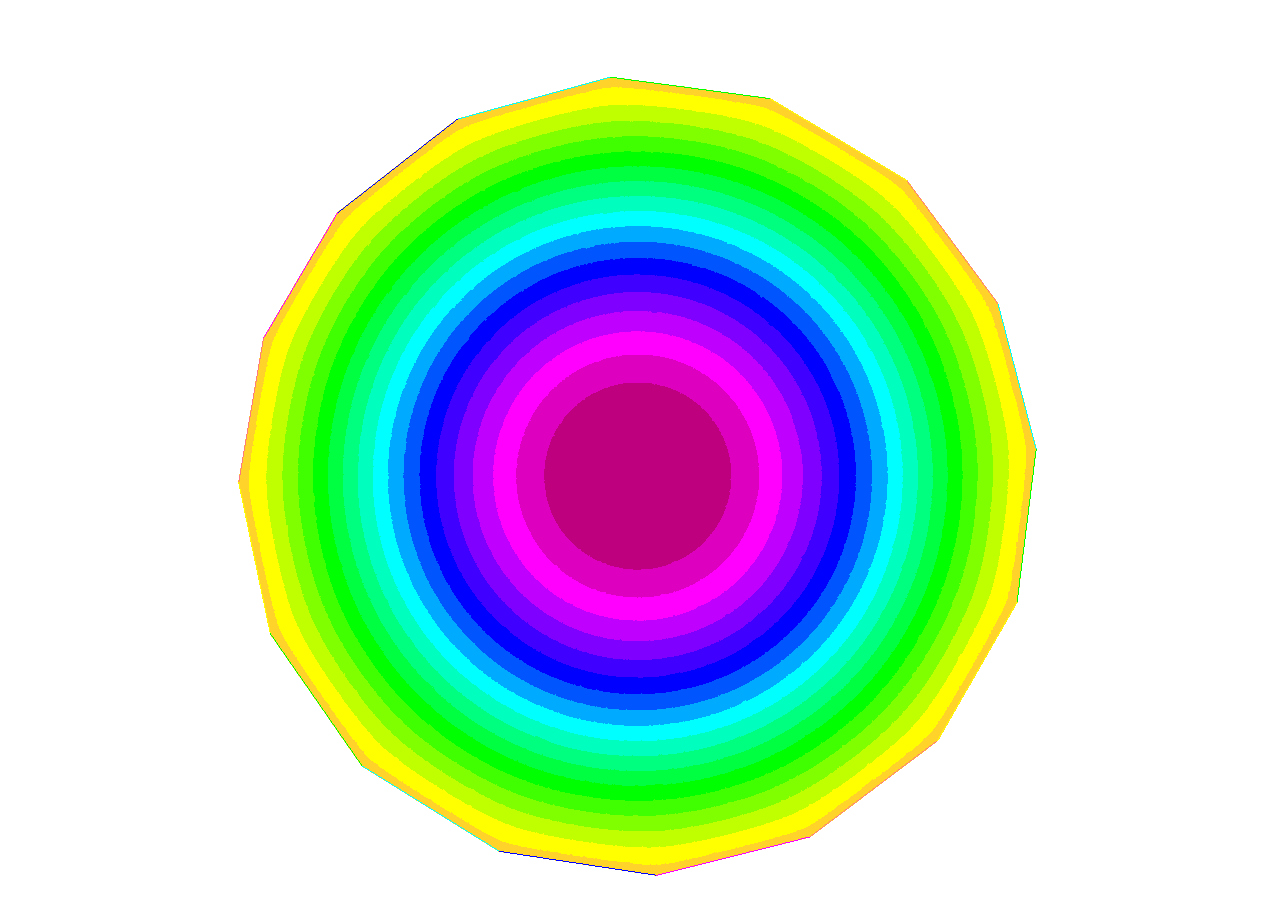
\includegraphics[width=0.5\textwidth]{16sides}
    }

    \subfloat[N = 17]{
        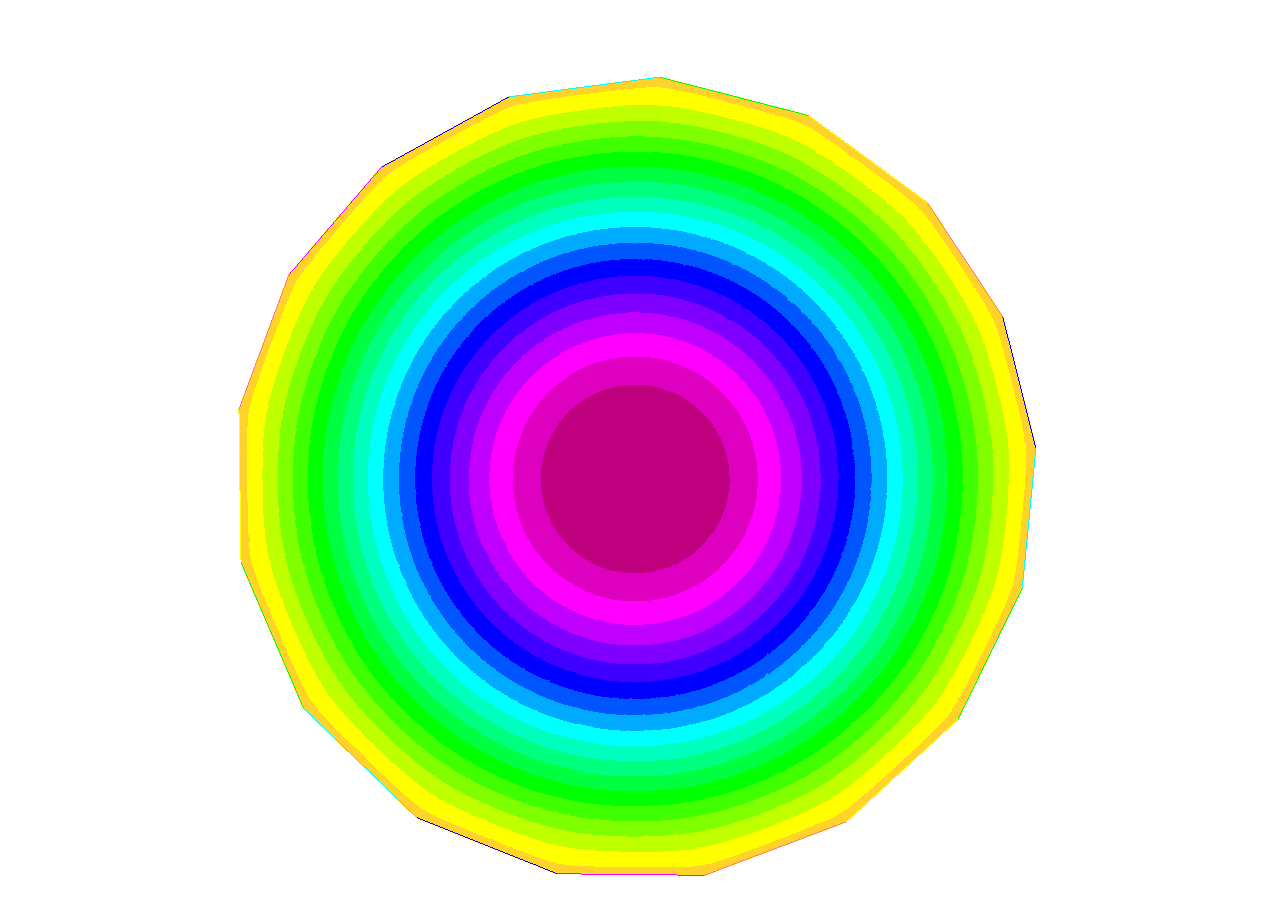
\includegraphics[width=0.5\textwidth]{17sides}
    }
    \subfloat[N = 18]{
        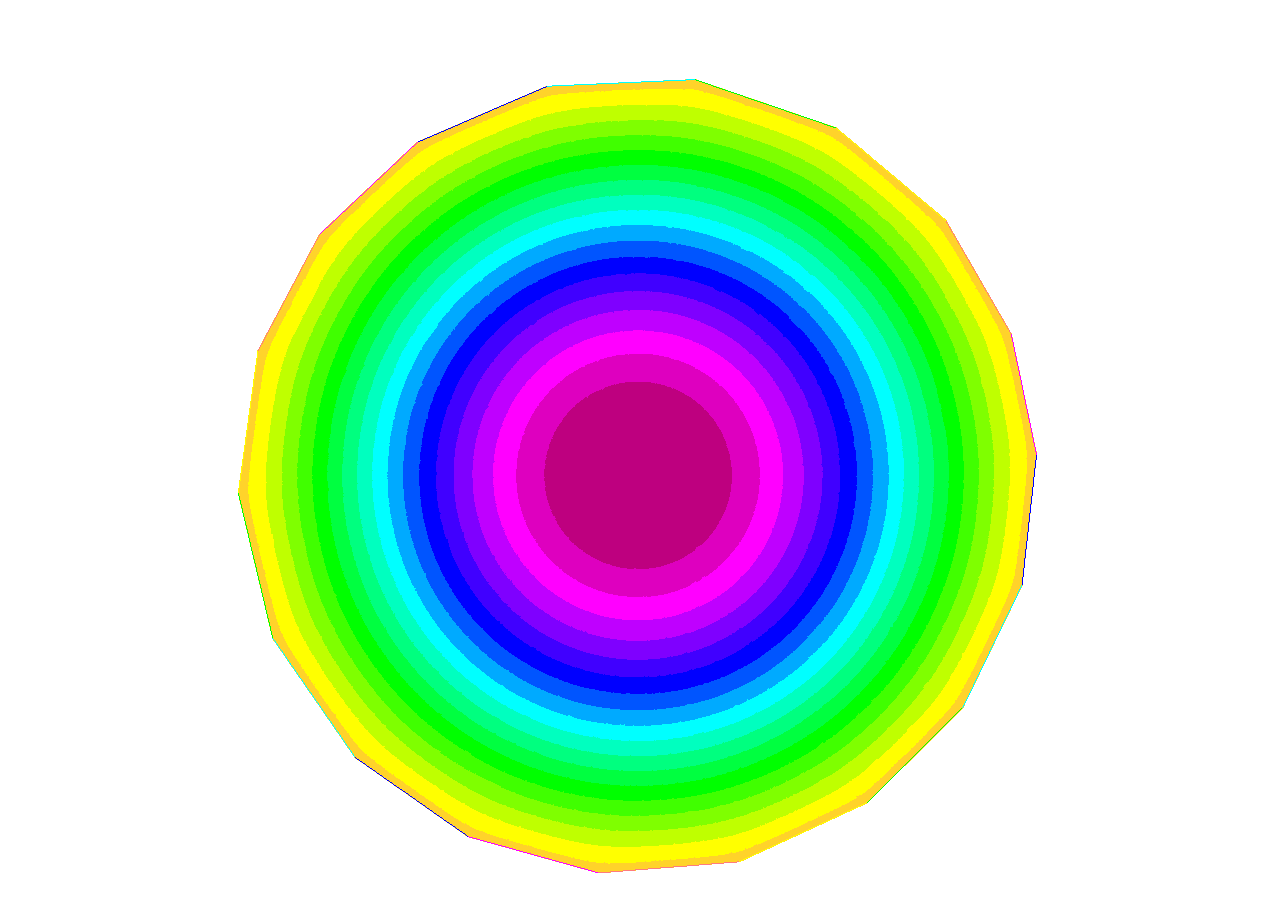
\includegraphics[width=0.5\textwidth]{18sides}
    }

    \caption{Domains and Eigenfunctions Obtained after $1000$ Iterations}
\end{figure}

\begin{figure}[hbt!]
    \centering

    \subfloat[N = 19]{
        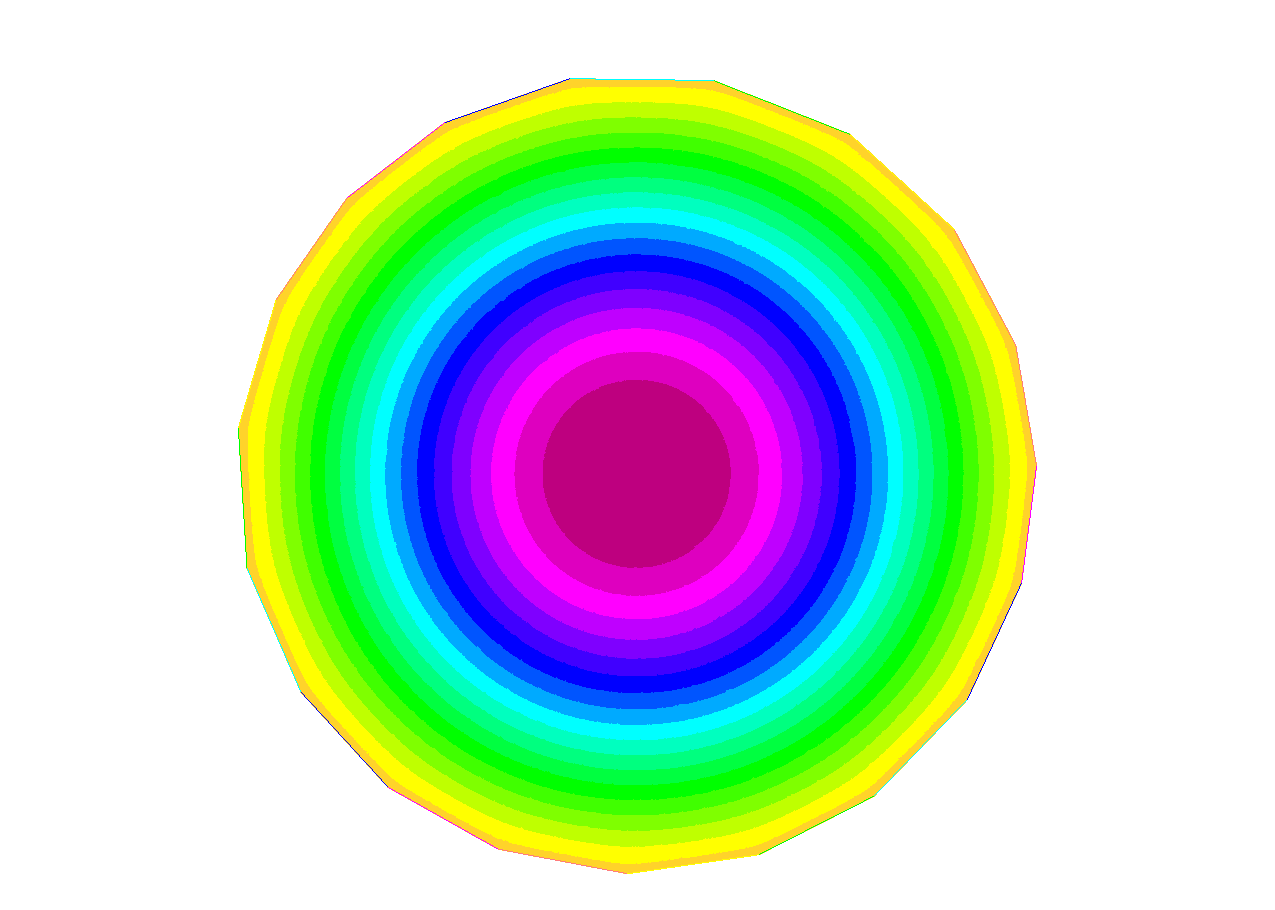
\includegraphics[width=0.5\textwidth]{19sides}
    }

    \subfloat[N = 20]{
        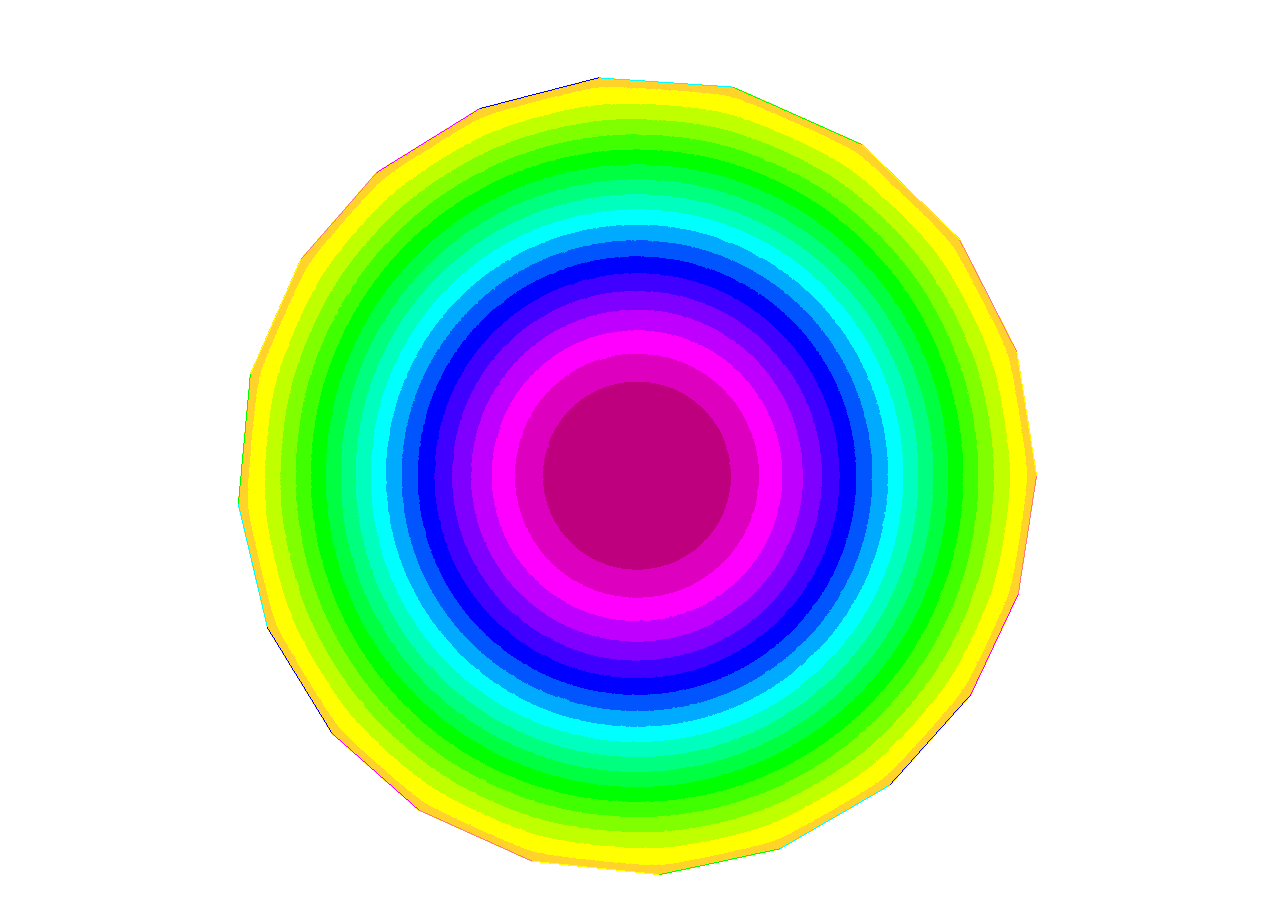
\includegraphics[width=0.5\textwidth]{20sides}
    }

    \subfloat[N = 21]{
        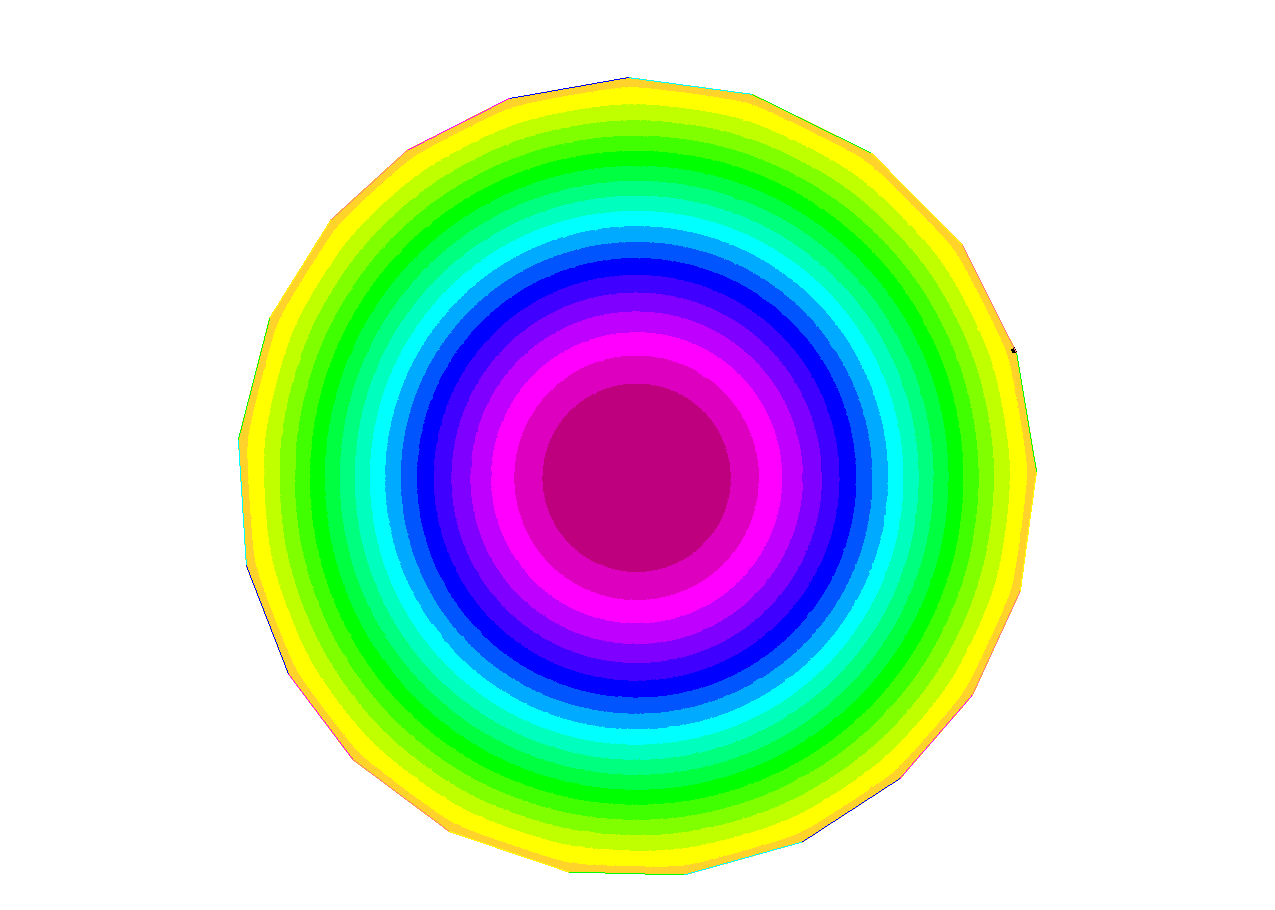
\includegraphics[width=0.5\textwidth]{21sides}
    }

    \subfloat[N = 22]{
        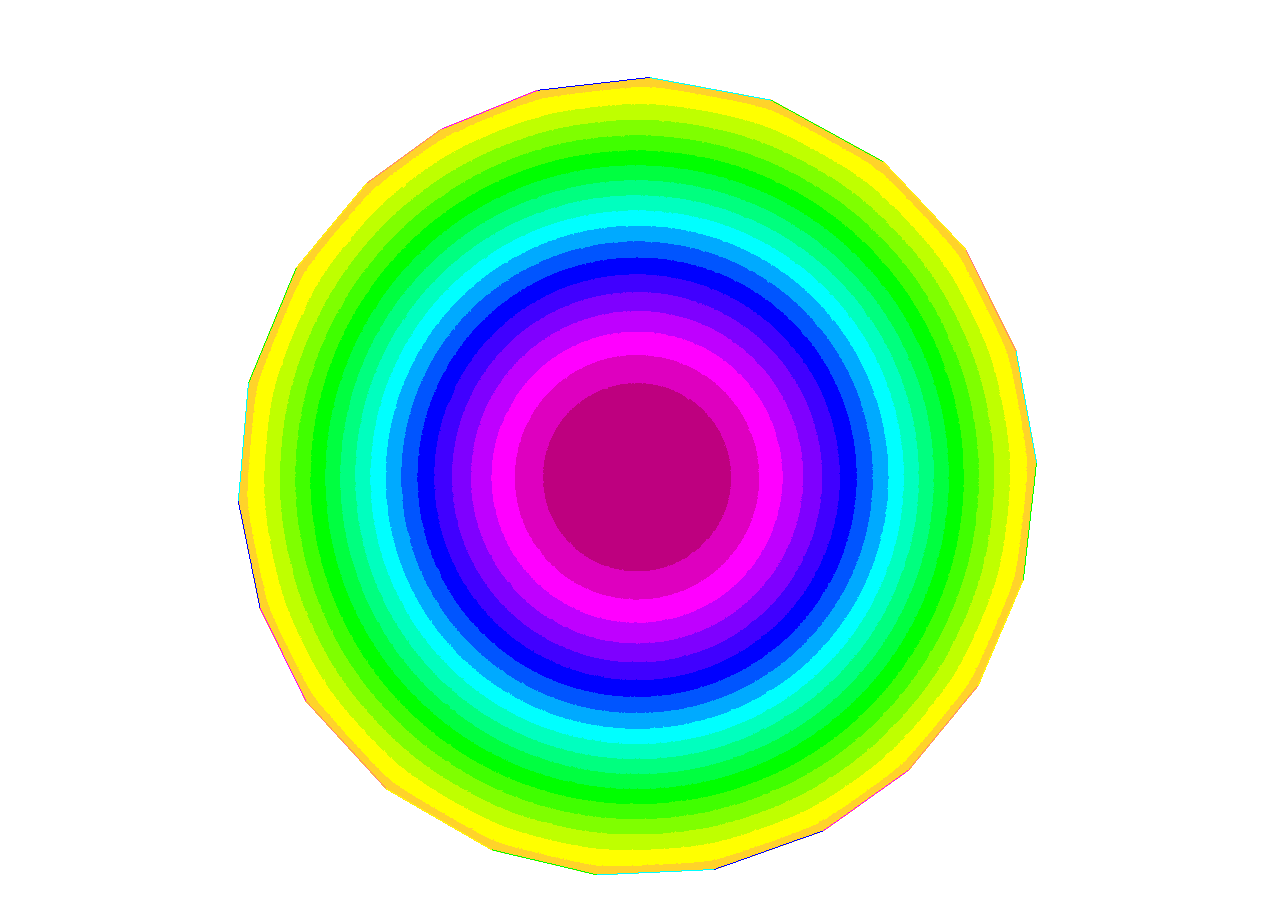
\includegraphics[width=0.5\textwidth]{22sides}
    }
    \subfloat[N = 23]{
        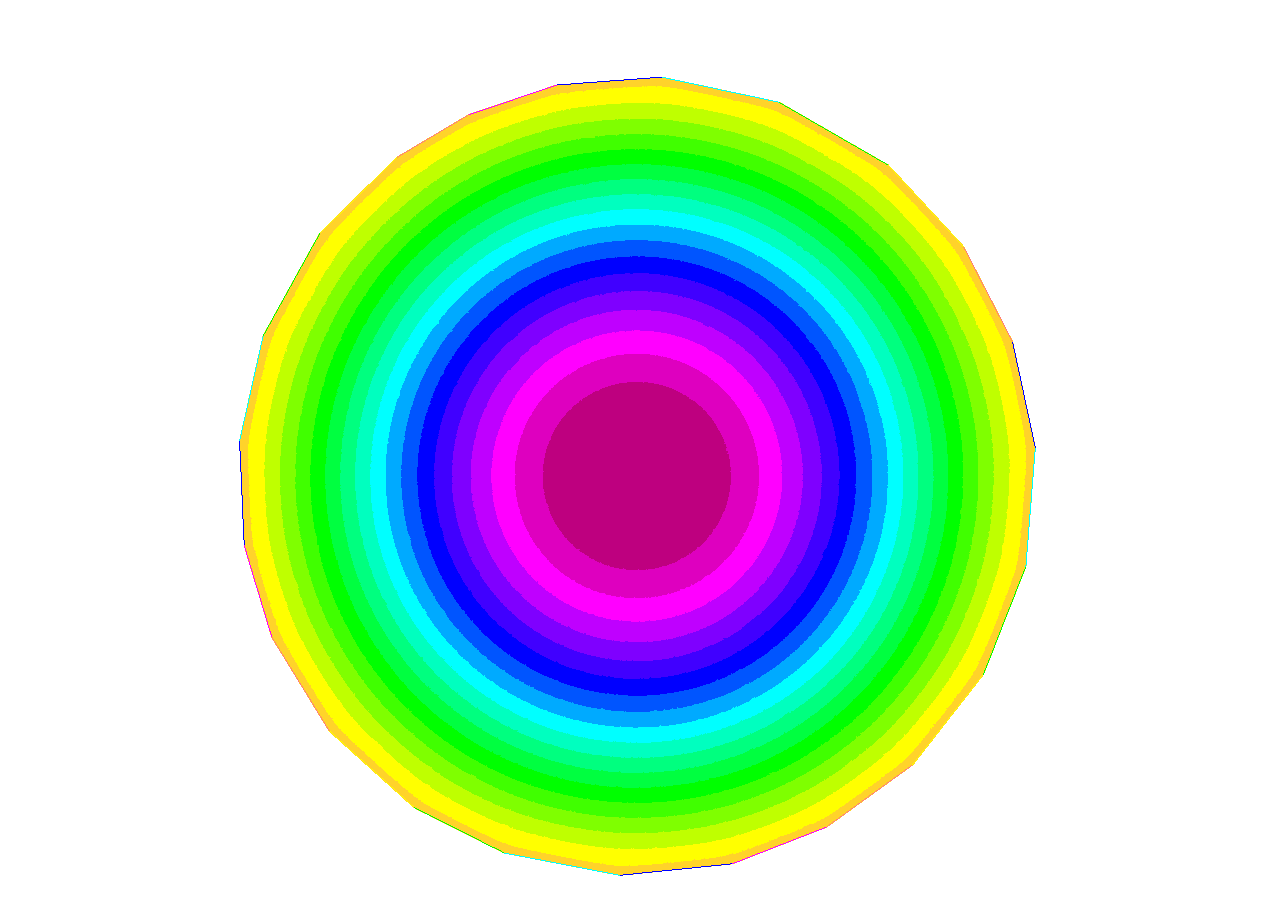
\includegraphics[width=0.5\textwidth]{23sides}
    }
    \caption{Domains and Eigenfunctions Obtained after $1000$ Iterations}
\end{figure}

  
% Only 1k iterations
\begin{landscape}
  \centering
  \begin{table}[ht] 
  \begin{tabular}{ c  c  c  c  c  c  c  c  c  c  c}
    \toprule
    \makecell{$N$} & \makecell{$| \Omega |^{2 / N}\lambda_{1}(\Omega)$} & \makecell{$| \Omega |\lambda_{1}(\Omega)$} & \makecell{$| \Omega | + \lambda_{1}(\Omega)$} & SD Edges & SD Angles & \makecell{$\lambda_{1}(\Omega)$} & \makecell{$|\Omega|$} & \makecell{$E_{max} - E_{min}$} & \makecell{$a_{max} - a_{min}$} & \makecell{$\lambda_{1}(\Omega)$; $| \Omega | = \pi$}  \\ [0.5ex]
    \midrule
    % NOTE: calculated fixed area by e.g. 4.82163 / (pi / 4.77054) ≈ 7.321693586
    $3$ & $13.6638$ & $23.0018$ & $9.59217$ & $0.000903421$ & $0.000471436$ & $4.82163$ & $4.77054$ &  $0.0018066$ &   $0.011993$ & $7.321693586$ \\
    $4$ & $9.47613$ & $19.8131$ & $8.90384$ & $0.00167785$ & $0.00116929$ &  $4.5322$ & $4.37164$ & $0.00301267$ &  $0.0117162$ & $6.306720505$ \\
    $5$ & $7.87774$ & $18.9617$ & $8.70924$ & $0.000782644$ & $0.00134324$ & $4.38616$ & $4.32309$ & $0.00167615$ & $0.00704458$ & $6.035717079$ \\
    $6$ & $7.06058$ & $18.6185$ & $8.63009$ &  $0.0111535$ & $0.00797373$ & $4.34799$ &  $4.2821$ &  $0.0165864$ & $0.00796461$ & $5.926461522$ \\
    $7$ & $6.53716$ & $18.4493$ & $8.59064$ & $0.00404326$ & $0.00428881$ & $4.31671$ & $4.27393$ &  $0.0106172$ & $0.00850759$ & $5.825175258$ \\
    $8$ & $6.18329$ & $18.3544$ & $8.56849$ & $0.00397916$ & $0.00325196$ & $4.30242$ & $4.26608$ &  $0.0125646$ & $0.00607772$ & $5.872599794$ \\
    $9$ & $5.91702$ & $18.3003$ & $8.55579$ & $0.00679178$ & $0.00487505$ &  $4.2855$ & $4.27029$ &   $0.013155$ &  $0.0110205$ & $5.842408593$ \\
    $10$ & $5.71869$ & $18.2644$ & $8.54739$ & $0.000289865$ & $0.00174915$ & $4.27779$ &  $4.2696$ & $0.00107659$ & $0.00183927$ & $5.813755696$ \\
    $11$ & $5.56344$ &  $18.241$ &  $8.5419$ & $0.00120196$ &  $0.0016105$ & $4.27309$ & $4.26881$ & $0.00185864$ & $0.00262753$ & $5.800965295$ \\
    $12$ & $5.43978$ & $18.2243$ & $8.53798$ & $0.00575083$ & $0.00502071$ & $4.27137$ & $4.26661$ & $0.00532735$ &   $0.013003$ & $5.794727394$ \\
    $13$ & $5.34295$ & $18.2126$ & $8.53525$ & $0.00569156$ & $0.00483002$ &  $4.2751$ & $4.26015$ & $0.00597858$ &  $0.0129977$ & $5.797240213$ \\
    $14$ & $5.25317$ & $18.2047$ & $8.53339$ &  $0.0257253$ &   $0.021836$ & $4.27033$ & $4.26306$ &  $0.0164521$ &  $0.0587004$ & $5.806293601$ \\
    $15$ &  $5.1842$ & $18.1974$ & $8.53169$ & $0.00126855$ & $0.00314971$ & $4.27352$ & $4.25817$ & $0.00304295$ & $0.00308773$ & $5.792404256$ \\
    $16$ & $5.11785$ & $18.1926$ & $8.53055$ & $0.00520303$ & $0.00483006$ & $4.26973$ & $4.26082$ &  $0.0042254$ &  $0.0122493$ & $5.789661457$ \\
    $17$ & $5.06643$ & $18.1888$ & $8.52967$ &  $0.0145499$ &   $0.012603$ & $4.27256$ & $4.25711$ & $0.00821058$ &  $0.0306817$ & $5.788634094$ \\
    $18$ & $5.01205$ & $18.1855$ &  $8.5289$ & $0.00313011$ & $0.00324541$ & $4.26631$ & $4.26259$ & $0.00375669$ & $0.00605722$ & $5.790868831$ \\
    $19$ & $4.96923$ & $18.1831$ & $8.52832$ &   $0.015598$ &  $0.0134338$ & $4.26589$ & $4.26243$ &  $0.0137619$ &  $0.0295824$ & $5.786708782$ \\
    $20$ & $4.92696$ &  $18.181$ & $8.52785$ & $0.00897166$ & $0.00782581$ & $4.26161$ & $4.26623$ &  $0.0158309$ &   $0.018117$ & $5.787846967$ \\
    $21$ & $4.88867$ & $18.1795$ &  $8.5275$ &  $0.0144342$ &  $0.0129941$ & $4.25745$ & $4.27004$ &   $0.020888$ &  $0.0286532$ & $5.787194724$ \\
    $22$ & $4.85587$ & $18.1782$ & $8.52719$ &  $0.0162601$ &  $0.0139256$ & $4.25539$ & $4.27181$ &  $0.0279232$ &  $0.0329481$ & $5.785929784$ \\
    $23$ &  $4.8261$ &  $18.177$ & $8.52693$ &  $0.0183518$ &  $0.0156802$ &  $4.2535$ & $4.27343$ &  $0.0291557$ &  $0.0350144$ & $5.786306361$ \\[1ex]
    \bottomrule
  \end{tabular}
  \caption{Results obtained after $1000$ Iterations}
\end{table}
\end{landscape}


\newgeometry{paper=letterpaper, left=1.5in,right=1in,top=1in,bottom=1in, footskip=0.25in}
